\documentclass[journal]{IEEEtran}
\usepackage[utf8]{inputenc}
\usepackage[T1]{fontenc}
\usepackage{cite}
\usepackage{amsmath,amssymb,amsfonts}
\usepackage{graphicx}
\usepackage{booktabs}
\usepackage{tabularx}
\usepackage{array}
\usepackage{url}
\usepackage{xcolor}

\begin{document}

\title{ A Longitudinal Review of Machine Learning for Batteries and Zn-ion Systems from Scholar Snapshots, 2022-2026 }

\author{ Melody Song }

\maketitle

\begin{abstract}
This review synthesizes 88 deduplicated papers retrieved from 47 monthly Google Scholar replay months between June 2022 and April 2026. The archive produced 138 query runs, 41 unique downloadable PDFs, and 37 full-text parseable documents, while 31 papers remained visible in all 17 quarterly snapshots. Across the corpus, the most persistent themes were Transport, Grid, and Applied Storage, State Estimation and Health Monitoring, and Charging, Control, and BMS. The resulting synthesis separates publication-year evolution from archive-visibility bias and shows a field that moved from battery-state estimation and control toward a broader mix of materials informatics, interpretable ML, and targeted Zn-ion studies.
\end{abstract}

\begin{IEEEkeywords}
battery informatics, machine learning, literature review, Zn-ion batteries, materials informatics
\end{IEEEkeywords}

\section{Introduction}
The archived Scholar replay provides a narrow but longitudinal window into how battery-related machine learning papers were surfaced over time. The query program started with battery machine learning and Zn-ion phrasing, then broadened toward materials informatics and state-of-health themes. Across the earlier publication years, representative papers \cite{participationofbattery2020,acceleratingfunctionalma2013,machinelearningbased2021,machinelearningsystems2018} captured battery-health estimation, grid participation, and cycle-life prediction, while later publications \cite{machinelearningdriven2025,recentadvancesin2025,interpretablemachinelear2025,datadrivenapproaches2024,predictivedesignof2024} introduced stronger materials-informatics, Zn-ion, and interpretable-model motifs. The value of the archive is therefore not just that it stores papers, but that it also preserves which papers stayed visible month after month.

\section{Review Methodology}
The review corpus was assembled from normalized monthly crawl outputs rather than from a direct bibliographic API. Each paper was deduplicated by a stable key derived from canonical URL, normalized title, and PDF hash when available. Full text was extracted from parseable PDFs; when extraction failed, the synthesis fell back to titles, snippets, venue strings, and crawl metadata. The quarter-level analysis therefore combines archive coverage with a document-quality filter and should be read as an evidence-weighted replay review. To avoid overstating novelty, the discussion below explicitly distinguishes publication-year evidence from replay visibility evidence.

The query program widened in stages. The 2022 schedule emphasized `battery machine learning` and `zinc ion battery machine learning`; 2023 added `machine learning for batteries`; 2024 introduced `battery materials informatics`; and 2025--2026 added `battery state of health machine learning` while keeping the earlier families in rotation. This staged broadening helps explain why later archive quarters contain more materials-discovery language even though many operational battery papers remained highly recurrent.

\begin{table}[t]
\caption{Query-program evolution used to build the replay archive.}
\label{tab:query_program}
\centering
\footnotesize
\begin{tabularx}{\linewidth}{lX}
\toprule
Year & Query families emphasized \\
\midrule
2022 & zinc ion battery machine learning (7); battery machine learning (7) \\
2023 & machine learning for batteries (12); zinc ion battery machine learning (12) \\
2024 & battery materials informatics (12); battery machine learning (12); zinc ion battery machine learning (12) \\
2025 & battery materials informatics (12); battery state of health machine learning (12); battery machine learning (12); zinc ion battery machine learning (12) \\
2026 & battery materials informatics (4); battery state of health machine learning (4); battery machine learning (4); zinc ion battery machine learning (4) \\
\bottomrule
\end{tabularx}
\end{table}

\section{Corpus Overview}
The archive yielded 88 unique papers, but quarter-level retrieval counts were larger because the replay repeatedly surfaced durable Scholar results. Quarterly unique-paper counts climbed from 34 in the smallest quarter to 82 in the densest quarter, while quarter-first additions ranged from 0 to 45. The recurring keywords batteries, materials, lithium-ion, estimation, state, health, zinc, models show that battery state estimation and applied management were the semantic baseline, even before the query set matured. This overview also highlights a structural feature of the replay: visibility accumulated around a relatively small set of persistent papers even as new queries broadened the archive. In other words, the archive stores both literature content and search-result inertia.

\begin{table}[t]
\caption{Quarter-level archive coverage summary.}
\label{tab:coverage}
\centering
\footnotesize
\begin{tabularx}{\linewidth}{lrrr}
\toprule
Quarter & Unique & New & Months \\
\midrule
2022-Q2 & 45 & 45 & 1 \\
2022-Q3 & 50 & 7 & 3 \\
2022-Q4 & 48 & 0 & 3 \\
2023-Q1 & 34 & 1 & 3 \\
2023-Q2 & 34 & 0 & 3 \\
2023-Q3 & 34 & 0 & 3 \\
2023-Q4 & 38 & 0 & 3 \\
2024-Q1 & 63 & 18 & 3 \\
2024-Q2 & 66 & 0 & 3 \\
2024-Q3 & 66 & 0 & 3 \\
2024-Q4 & 66 & 0 & 3 \\
2025-Q1 & 82 & 16 & 3 \\
2025-Q2 & 82 & 1 & 3 \\
2025-Q3 & 82 & 0 & 3 \\
2025-Q4 & 77 & 0 & 3 \\
2026-Q1 & 82 & 0 & 3 \\
2026-Q2 & 72 & 0 & 1 \\
\bottomrule
\end{tabularx}
\end{table}

\begin{figure}[t]
\centering
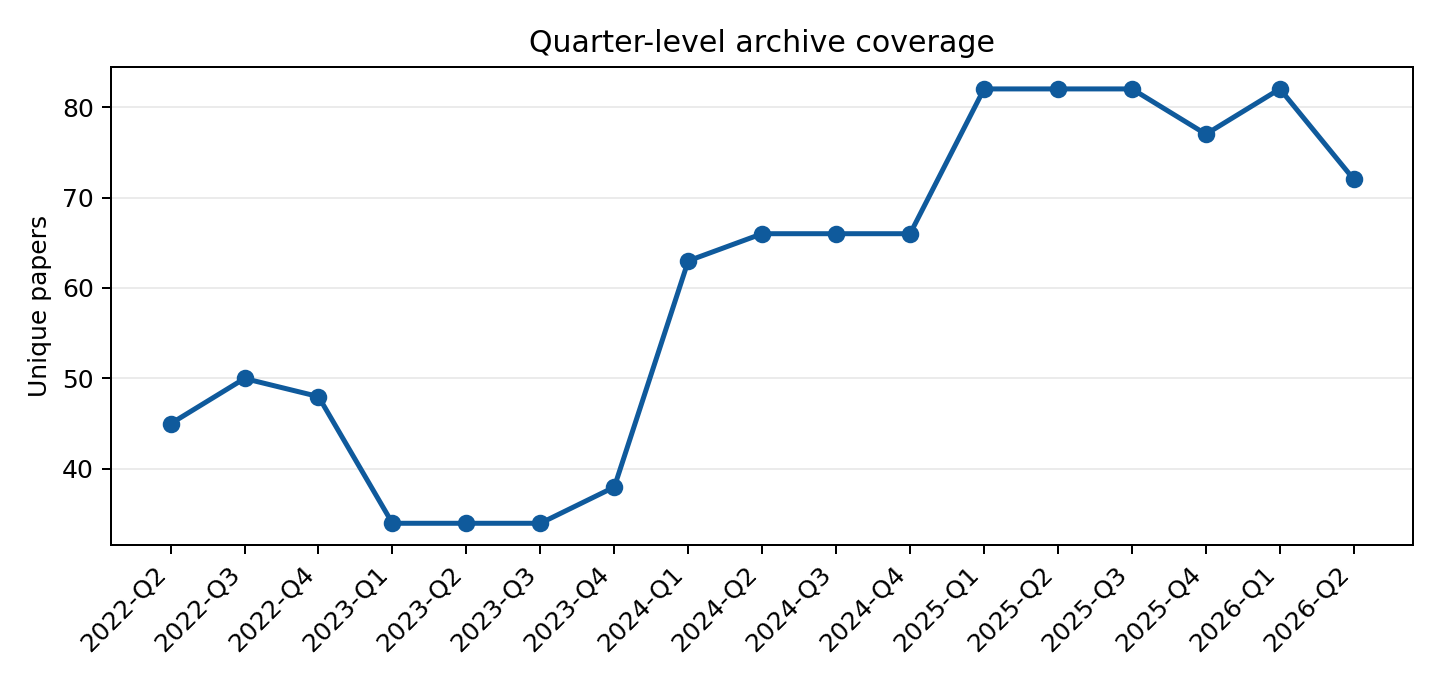
\includegraphics[width=\linewidth]{figures/quarter_counts.png}
\caption{Unique papers retrieved in each quarterly archive snapshot.}
\label{fig:quarter_counts}
\end{figure}

\begin{figure}[t]
\centering
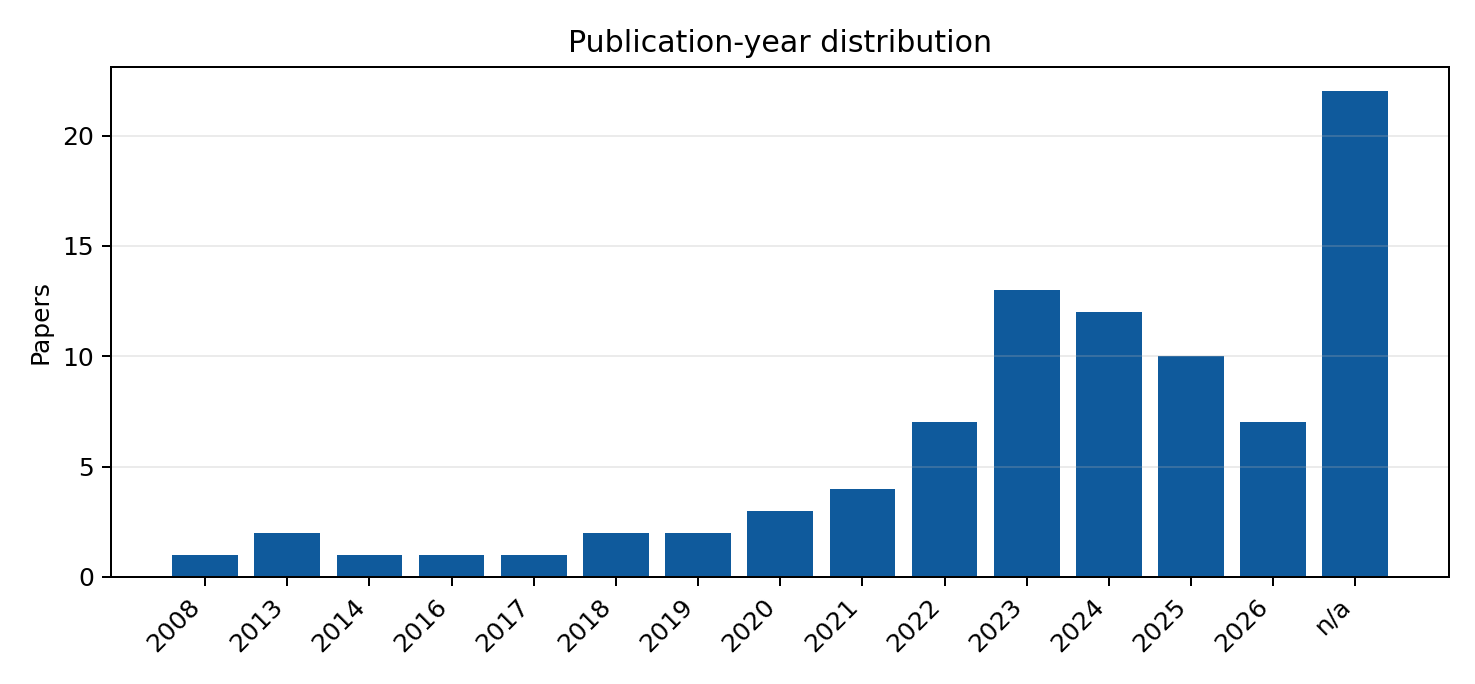
\includegraphics[width=\linewidth]{figures/publication_year_counts.png}
\caption{Publication-year distribution for papers retained in the deduplicated corpus.}
\label{fig:publication_years}
\end{figure}

\section{Archive Visibility and Source Bias}
Visibility persistence is one of the archive's strongest signals. 31 papers remained visible in all 17 quarters, and 66 were still present in at least 10 quarters. That persistence means the replay behaves less like a fresh literature search every month and more like a ranking memory of what Google Scholar repeatedly surfaced. The host distribution sharpens this interpretation further: the largest source groups were social scholar networks (44), publisher and proceedings hosts (15), institutional repositories (11), yet the accessibility profile was uneven. Social scholar networks contributed 44 papers but yielded essentially no parseable full-text documents in the normalized corpus, whereas institutional repositories contributed only 11 papers but converted into 10 downloadable PDFs and 9 full-text extractions.

\begin{table}[t]
\caption{Host-group composition and document accessibility.}
\label{tab:source_bias}
\centering
\footnotesize
\begin{tabularx}{\linewidth}{Xrrr}
\toprule
Host group & Papers & PDFs & Full text \\
\midrule
Social scholar network & 44 & 1 & 1 \\
Publisher or proceedings host & 15 & 13 & 11 \\
Institutional repository & 11 & 10 & 9 \\
Other host & 11 & 10 & 9 \\
Preprint or project host & 7 & 7 & 7 \\
\bottomrule
\end{tabularx}
\end{table}

\begin{figure}[t]
\centering
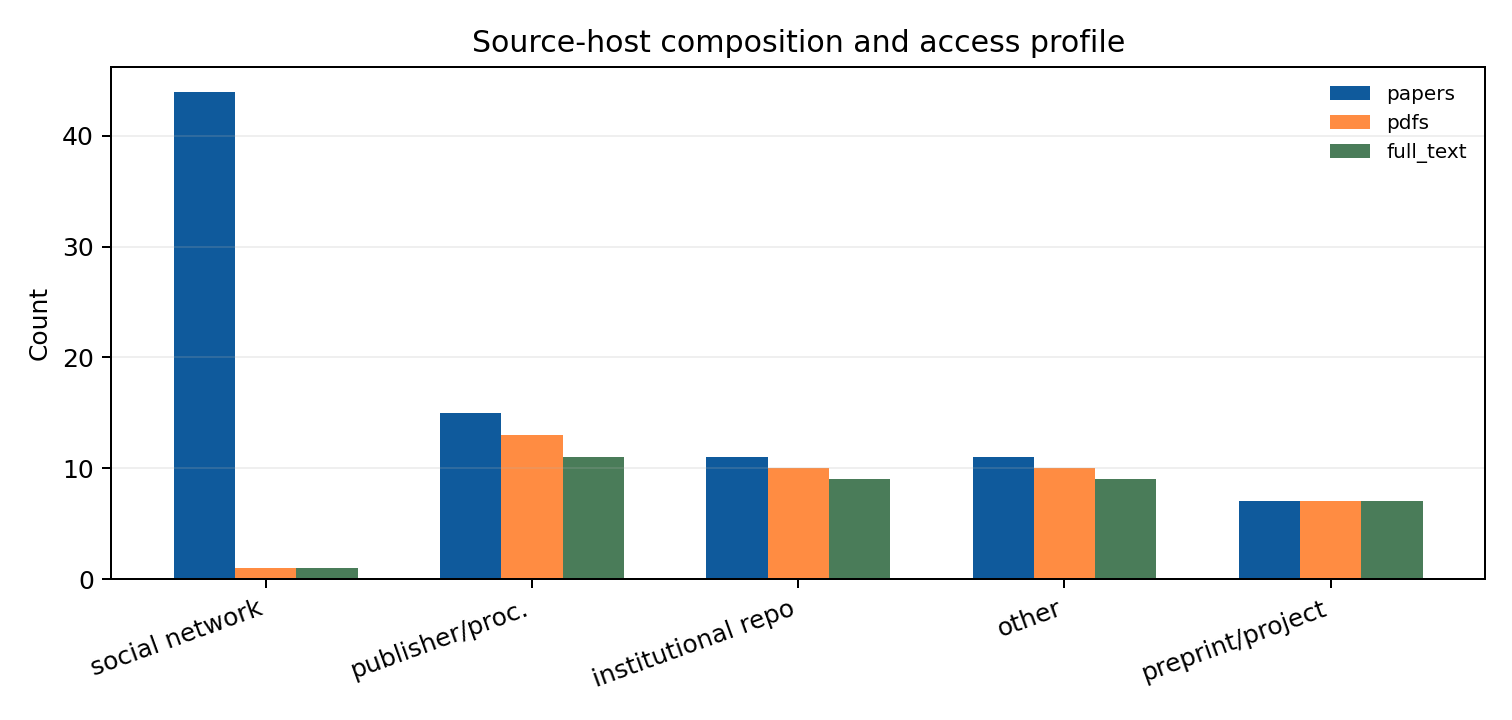
\includegraphics[width=\linewidth]{figures/host_group_counts.png}
\caption{Source-host groups and document accessibility across the archive.}
\label{fig:host_groups}
\end{figure}

\begin{table}[t]
\caption{Most persistent results in the replay archive.}
\label{tab:visibility}
\centering
\footnotesize
\begin{tabularx}{\linewidth}{p{0.5\linewidth} rr}
\toprule
Paper & Months seen & Retrievals \\
\midrule
\textit{Battery detection of XRay images using transfer learning} & 45 & 90 \\
\textit{An effective approach towards battery using Artificial Inte...} & 45 & 85 \\
\textit{Battery health monitoring using machine learning} & 45 & 60 \\
\textit{Data-driven approaches to battery health monitoring in elec...} & 45 & 60 \\
\textit{Machine Learning and Cloud Technologies for Control and Sta...} & 45 & 60 \\
\textit{Dimensionality reduced deep learning-based state of health...} & 45 & 56 \\
\textit{A Physics-Inspired Machine Learning Nonlinear Model of Li-i...} & 45 & 45 \\
\textit{AI-Driven Screening of Electrolyte Additives for Aqueous Zi...} & 45 & 45 \\
\bottomrule
\end{tabularx}
\end{table}

\section{Topical Taxonomy}
The dominant thematic families were Transport, Grid, and Applied Storage (66), State Estimation and Health Monitoring (44), Charging, Control, and BMS (42), Materials Informatics and Discovery (34), Interpretability and Diagnostics (18). Health-oriented work \cite{stateestimationof2023,onlineconditionmonitorin2022,socestimationof2023,participationofbattery2020} remained central throughout the archive, while charging and BMS studies \cite{stateestimationof2023,onlineconditionmonitorin2022,socestimationof2023,participationofbattery2020} formed a second stable core. Materials-informatics papers \cite{textminingfor2022,recentadvancesin2025,interpretablemachinelear2025,datadrivenapproaches2024} became more visible in the 2024--2026 portion of the archive, and explicit Zn-ion coverage \cite{recentadvancesin2025,predictivedesignof2024,electrolytesforaqueous2025} was present but comparatively sparse. The taxonomy therefore points to a field that expanded by layering discovery-oriented work onto an already mature diagnostics and control base. Knowledge-graph and text-mining work \cite{textminingfor2022,acceleratingfunctionalma2013} was rare but conceptually important because it suggested a shift from single-task predictors toward broader battery-information infrastructures.

\begin{table}[t]
\caption{Dominant topical and model categories in the full archive.}
\label{tab:taxonomy}
\centering
\footnotesize
\begin{tabularx}{\linewidth}{XrXr}
\toprule
Topic cluster & Count & Model family & Count \\
\midrule
Transport, Grid, and Applied Storage & 66 & Unspecified or Broad ML & 43 \\
State Estimation and Health Monitoring & 44 & Neural and Deep Models & 33 \\
Charging, Control, and BMS & 42 & Kernel and Linear Models & 21 \\
Materials Informatics and Discovery & 34 & Tree and Boosting Models & 12 \\
Interpretability and Diagnostics & 18 & Gaussian and Bayesian Models & 10 \\
\bottomrule
\end{tabularx}
\end{table}

\begin{figure}[t]
\centering
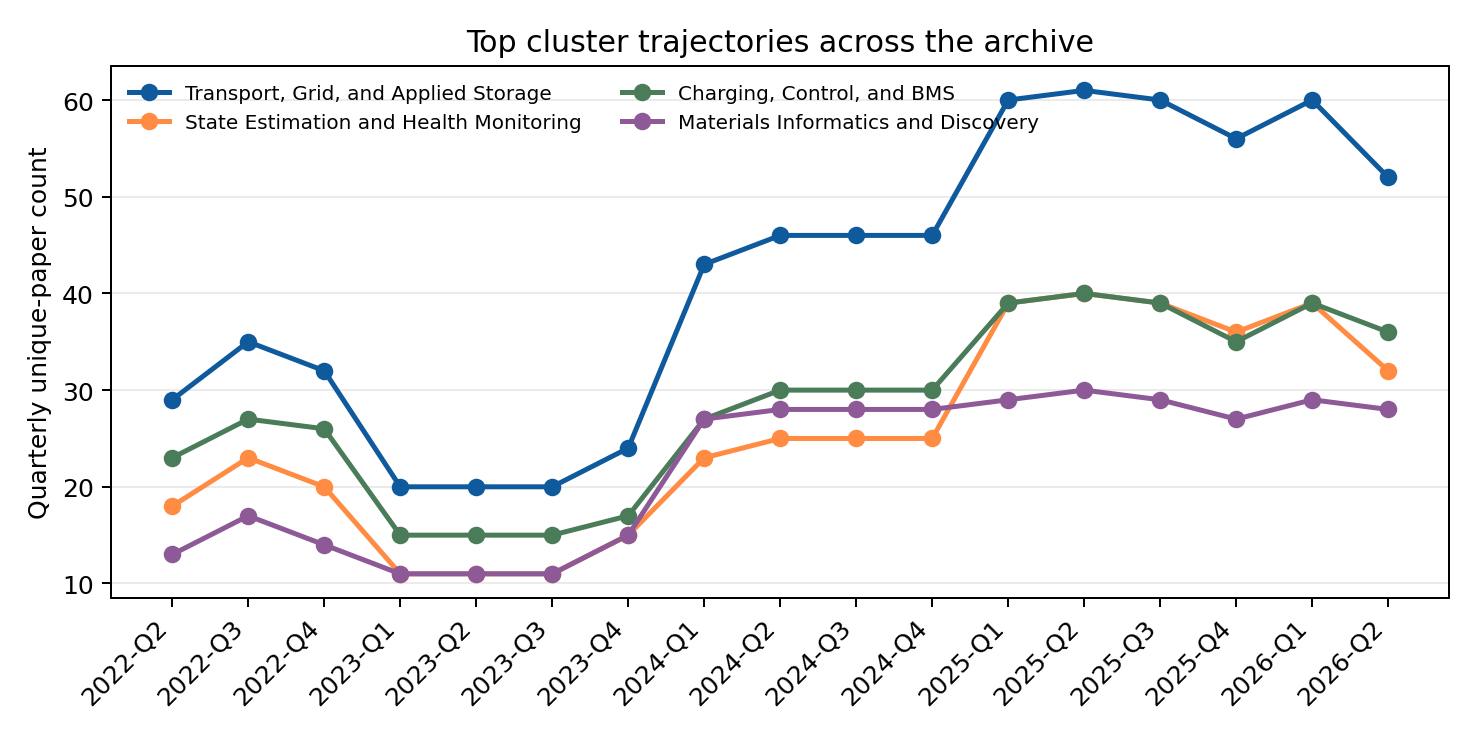
\includegraphics[width=\linewidth]{figures/cluster_trends.png}
\caption{Quarter-level counts for the dominant topic clusters.}
\label{fig:cluster_trends}
\end{figure}

\section{Methods Landscape}
The methods profile was led by Unspecified or Broad ML (43), Neural and Deep Models (33), Kernel and Linear Models (21), Tree and Boosting Models (12), Gaussian and Bayesian Models (10). In practical terms, the archive often described machine learning broadly without naming the full modeling stack, but identifiable families still showed a shift from classical predictive models toward deeper architectures, interpretable AI, and physics-guided variants. The interpretability layer was visible in at least 2 title-or-snippet records and is represented directly by papers such as \cite{stateestimationof2023,onlineconditionmonitorin2022,socestimationof2023,machinelearningdriven2025}. This suggests that the vocabulary of the field matured faster than the metadata quality of the archived search results.

\begin{figure}[t]
\centering
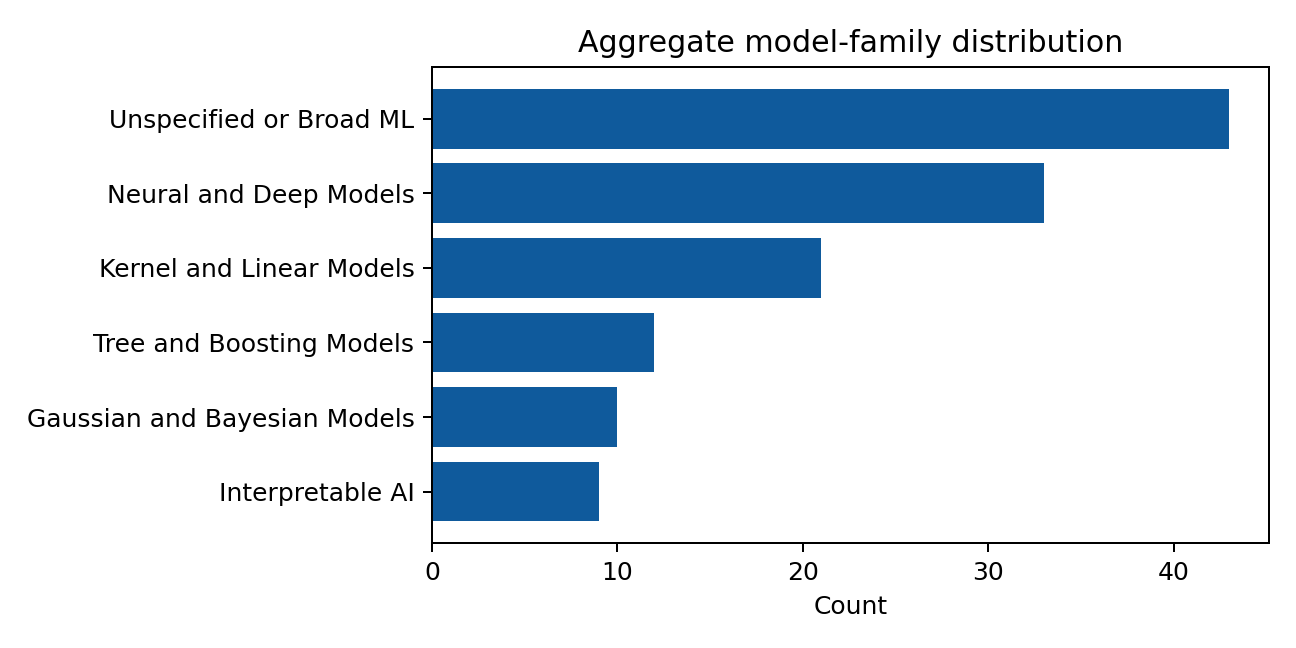
\includegraphics[width=\linewidth]{figures/model_families.png}
\caption{Aggregate model-family distribution across the deduplicated archive.}
\label{fig:model_families}
\end{figure}

\section{Operational Battery Analytics}
Operational battery analytics was the stable center of gravity throughout the archive. In title-and-snippet space alone, 8 papers referenced state-of-charge style language, 16 referenced state-of-health, 4 pointed to cycle-life or remaining-life tasks, 10 directly named battery-management workflows, and 3 mentioned thermal behavior or safety proxies. Those counts align with the representative operational papers \cite{stateestimationof2023,onlineconditionmonitorin2022,socestimationof2023,participationofbattery2020} and \cite{stateestimationof2023,onlineconditionmonitorin2022,socestimationof2023,participationofbattery2020}, which repeatedly framed machine learning as a tool for estimation, control, balancing, monitoring, and fault-sensitive operation. Digital-twin language appeared in 1 papers, suggesting that the field's operational branch increasingly sought richer system representations rather than only point predictions.

\section{Materials Informatics and Zn-ion Coverage}
Materials-oriented and Zn-ion-oriented work formed the archive's most visible expansion front. Across the deduplicated corpus, 19 papers used materials-discovery language in titles or snippets, while 8 explicitly referenced Zn-ion or aqueous-zinc systems. The most informative materials and Zn-ion anchors \cite{textminingfor2022,recentadvancesin2025,interpretablemachinelear2025,datadrivenapproaches2024} and \cite{recentadvancesin2025,predictivedesignof2024,electrolytesforaqueous2025} reveal two related shifts: first, battery ML began to speak more often about cathodes, electrolytes, and surrogate-guided screening; second, Zn-ion coverage emerged as a specialized but persistent substream rather than a dominant branch. This means the archive does not support a claim that Zn-ion became central, but it does support the weaker and more accurate claim that Zn-ion themes became a recognizable edge case within the broader rise of battery materials informatics.

\section{Knowledge Progression by Era}
The publication-year view supports a three-era reading. The foundational era \cite{participationofbattery2020,acceleratingfunctionalma2013,machinelearningbased2021,machinelearningsystems2018} was dominated by operational estimation, grid participation, and early machine-learning deployments around lithium-ion systems. The transition era \cite{stateestimationof2023,onlineconditionmonitorin2022,socestimationof2023,textminingfor2022} broadened toward BMS framing, comparative modeling studies, and stronger state-estimation language. The recent expansion era \cite{machinelearningdriven2025,recentadvancesin2025,interpretablemachinelear2025,datadrivenapproaches2024,predictivedesignof2024} did not displace those operational concerns, but it added more materials-informatics, Zn-ion, and interpretability motifs. That pattern matters because it suggests accumulation rather than replacement: newer battery-ML knowledge seems to stack additional discovery and explanation goals on top of an enduring operations core.

\begin{table}[t]
\caption{Publication-era summary across the deduplicated corpus.}
\label{tab:era_summary}
\centering
\footnotesize
\begin{tabularx}{\linewidth}{lrrXX}
\toprule
Era & Papers & PDFs & Dominant clusters & Dominant models \\
\midrule
Foundational (2008-2021) & 17 & 8 & Transport, Grid, and Applied Storage (13), State Estimation and Health Monitoring (10) & Unspecified or Broad ML (8), Neural and Deep Models (6) \\
Transition (2022-2023) & 20 & 10 & Transport, Grid, and Applied Storage (16), Charging, Control, and BMS (13) & Unspecified or Broad ML (10), Neural and Deep Models (9) \\
Recent expansion (2024-2026) & 29 & 13 & Transport, Grid, and Applied Storage (21), Materials Informatics and Discovery (17) & Unspecified or Broad ML (15), Neural and Deep Models (12) \\
Undated archive-only & 22 & 10 & Transport, Grid, and Applied Storage (16), State Estimation and Health Monitoring (10) & Unspecified or Broad ML (10), Kernel and Linear Models (7) \\
\bottomrule
\end{tabularx}
\end{table}

\section{Cross-cutting Battery Findings}
Viewed across all sections, the archive suggests five cross-cutting findings. First, battery ML remained overwhelmingly application-led rather than method-led. Second, the most stable problems were still health estimation, control, and management in vehicle or storage contexts. Third, materials informatics emerged as the clearest late-stage expansion route. Fourth, Zn-ion work was visible enough to matter but not numerous enough to dominate. Fifth, archive visibility and document access significantly shaped the apparent literature map. The representative anchor papers in Table~\ref{tab:synthesis_anchors} therefore should be read not only as technical exemplars, but also as evidence of what the replay made historically visible.

\begin{table}[t]
\caption{Representative papers used to anchor the synthesis narrative.}
\label{tab:synthesis_anchors}
\centering
\footnotesize
\begin{tabularx}{\linewidth}{p{0.44\linewidth} p{0.12\linewidth} X}
\toprule
Paper & Year & Role in synthesis \\
\midrule
\textit{State Estimation of Li-ion Batteries Using Machine Le...} \cite{stateestimationof2023} & 2023 & State Estimation and Health Monitoring, Neural and Deep Models \\
\textit{Online Condition Monitoring and Health Management of...} \cite{onlineconditionmonitorin2022} & 2022 & State Estimation and Health Monitoring, Neural and Deep Models \\
\textit{SoC estimation of Lithium-ion battery: Simulation and...} \cite{socestimationof2023} & 2023 & State Estimation and Health Monitoring, Unspecified or Broad ML \\
\textit{Participation of battery storage systems in the autom...} \cite{participationofbattery2020} & 2020 & State Estimation and Health Monitoring, Neural and Deep Models \\
\textit{Machine learning-driven material intelligence researc...} \cite{machinelearningdriven2025} & 2025 & Charging, Control, and BMS, Neural and Deep Models \\
\textit{Text Mining for Energy Materials} \cite{textminingfor2022} & 2022 & State Estimation and Health Monitoring, Neural and Deep Models \\
\textit{Recent advances in MXene materials for zinc-ion hybri...} \cite{recentadvancesin2025} & 2025 & State Estimation and Health Monitoring, Unspecified or Broad ML \\
\textit{Interpretable machine learning for battery health ins...} \cite{interpretablemachinelear2025} & 2025 & State Estimation and Health Monitoring, Neural and Deep Models \\
\textit{Data-driven approaches to battery health monitoring i...} \cite{datadrivenapproaches2024} & 2024 & State Estimation and Health Monitoring, Neural and Deep Models \\
\textit{Predictive Design of Ultrastretchable Electrodes with...} \cite{predictivedesignof2024} & 2024 & Charging, Control, and BMS, Neural and Deep Models \\
\bottomrule
\end{tabularx}
\end{table}

\paragraph{State Estimation of Li-ion Batteries Using Machine Learning Algorithms} As a synthesis anchor, this paper represents state estimation and health monitoring and is associated with neural and deep models, kernel and linear models. ... measurements for states estimation of Li-ion batteries using different machine learning (ML) ... utilized for estimating two of the most important states of Li-ion batteries, ie, SOC and SOH. ... \cite{stateestimationof2023}

\paragraph{Online Condition Monitoring and Health Management of Batteries Based on D...} As a synthesis anchor, this paper represents state estimation and health monitoring and is associated with neural and deep models, kernel and linear models. ... health indicators from CC charging voltages for battery SOH ... are highly correlated with the battery SOH. The results reveal ... Then two different machine learning models are introduced ... \cite{onlineconditionmonitorin2022}

\paragraph{SoC estimation of Lithium-ion battery: Simulation and Comparative study o...} As a synthesis anchor, this paper represents state estimation and health monitoring and is associated with unspecified or broad ml. ... battery. The Scikitlearn library in Python helped us to develop the different machine learning ... analyze the feasibility of using different machine learning methods in the estimation of SoC. ... \cite{socestimationof2023}

\paragraph{Participation of battery storage systems in the automatic frequency resto...} As a synthesis anchor, this paper represents state estimation and health monitoring and is associated with neural and deep models. ... Both statistical and machine learning based models are ... strategy for integrating Battery Energy Storage Systems (BESS) ... An in-depth cost breakdown and battery-ageing model support ... \cite{participationofbattery2020}

\paragraph{Machine learning-driven material intelligence research and development} As a synthesis anchor, this paper represents charging, control, and bms and is associated with neural and deep models, tree and boosting models. ... [164] achieves cross screening of lithium/zinc/aluminum ion batteries positive electrode materials (MAE 47.34 Whkg1) through the autoencoder Coulomb matrix and CNN model. Its ... \cite{machinelearningdriven2025}

\paragraph{Text Mining for Energy Materials} As a synthesis anchor, this paper represents state estimation and health monitoring and is associated with neural and deep models, kernel and linear models. ... The applications of the text mining method for energy materials, including thermoelectric materials, solar cell materials, battery materials, materials for hydrogen fuels and catalyst are ... \cite{textminingfor2022}

\paragraph{Recent advances in MXene materials for zinc-ion hybrid capacitors} As a synthesis anchor, this paper represents state estimation and health monitoring and is associated with unspecified or broad ml. ... Common ZHCs are a compromise between zinc ion batteries and supercapacitors, where the battery-type anode stores a large amount of energy through redox reactions and the ... \cite{recentadvancesin2025}

\paragraph{Interpretable machine learning for battery health insights: A LIME and SH...} As a synthesis anchor, this paper represents state estimation and health monitoring and is associated with neural and deep models, tree and boosting models. ... study of interpretable machine learning methods for lithium-ion battery state of health (SOH) ... transparent, trustworthy SOH estimators into safety-critical battery management systems. ... \cite{interpretablemachinelear2025}

\paragraph{Data-driven approaches to battery health monitoring in electric vehicles...} As a synthesis anchor, this paper represents state estimation and health monitoring and is associated with neural and deep models, tree and boosting models. ... apply innovative machinelearning techniques to battery health estimation ... machine learning to battery health monitoring, will guide the vehicle driver to action in ways implicit for battery ... \cite{datadrivenapproaches2024}

\paragraph{Predictive Design of Ultrastretchable Electrodes with Strain-Insensitive...} As a synthesis anchor, this paper represents charging, control, and bms and is associated with neural and deep models. ... gold conductors, a Zn//MnO2 battery was fabricated and showcased ... Our machine intelligence workflow realized a predictive ... and stretchable zinc ion batteries. ACS Appl. Energy Mater. ... \cite{predictivedesignof2024}

\paragraph{Electrolytes for aqueous Zn-ion batteries working in harsh environment: a...} As a synthesis anchor, this paper represents state estimation and health monitoring and is associated with unspecified or broad ml. ... plating/stripping performance of Zn||Zn batteries with BBAS ... electrolyte facilitates the ultra-stable Zn||Zn cell at 1 mA cm2 over ... polyol in the solvation structure of zinc ions reduces water ... \cite{electrolytesforaqueous2025}

\paragraph{Accelerating functional materials discovery Insights from geological scie...} As a synthesis anchor, this paper represents state estimation and health monitoring and is associated with interpretable ai. ... materials synthesis, characterization, theory, and high-throughput combinatorial and informatics ... of LixCoO2 (which is the primary cathode material in lithium-ion batteries) as well as the ... \cite{acceleratingfunctionalma2013}

\section{Temporal Trends 2022--2026}
If the archive is read simultaneously as a literature sample and a search-visibility record, the temporal story becomes more credible. The query program broadened every one to two years, the later publication years injected more materials and Zn-ion language, and the archive nonetheless kept resurfacing a stable operational core. That combination explains why the quarter plots show continuity even while the publication-year analysis shows expansion: Scholar visibility had inertia, but the knowledge frontier still widened.

\section{Limitations}
This review inherits the biases of the Scholar replay. Papers with accessible PDFs are overrepresented, repeated high-ranking results persist across months, and several quarters mix publication years because retrieval time and publication time are not the same event. Moreover, only 37 papers supplied reliable full text, so some of the synthesis rests on snippet-level evidence instead of complete manuscripts. The source-bias results in Table~\ref{tab:source_bias} should therefore be treated as part of the finding, not just as noise.

\section{Future Directions}
A natural next step is to combine the replay archive with cleaner bibliographic metadata, citation graphs, and venue normalization. For the battery domain itself, the most interesting forward-looking seam is the bridge between operational battery diagnostics and materials discovery: the archive now contains enough evidence to study whether those once-separate tracks are converging around shared surrogate models, interpretability tools, and data engineering practices. A second next step is methodological: a richer replay should preserve ranking position, all-versions links, and citation counts so that future syntheses can separate scientific importance from search visibility more convincingly.

\section{Conclusion}
Across 2022--2026, the archive describes a battery-ML landscape that broadened rather than simply scaled. Health monitoring and control remained foundational, materials informatics rose steadily, and Zn-ion work persisted as a targeted but smaller slice of the literature. The quarterly replay format therefore works well as a historical lens: it preserves both the repetition of highly visible papers and the gradual widening of the field. The longer view offered here is that the archive captures a field in layered expansion, where new chemical systems, new model families, and new data infrastructures accumulated on top of an operational battery-analytics base rather than replacing it.

\bibliographystyle{IEEEtran}
\bibliography{references}

\end{document}